\subsection{Operationsverstärker}
	\subsection{Schaltbilder}

	\begin{figure}[h]
	\begin{subfigure}{0.25\textwidth}
		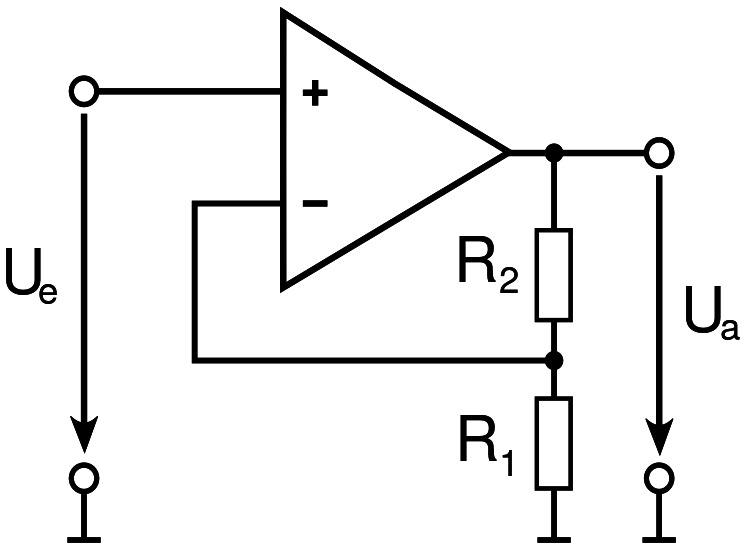
\includegraphics[width=\textwidth]{images/Noninverting_Amplifier}
		\caption{Nicht invertierender Verstärker}
	\end{subfigure}
	\begin{subfigure}{0.25\textwidth}
		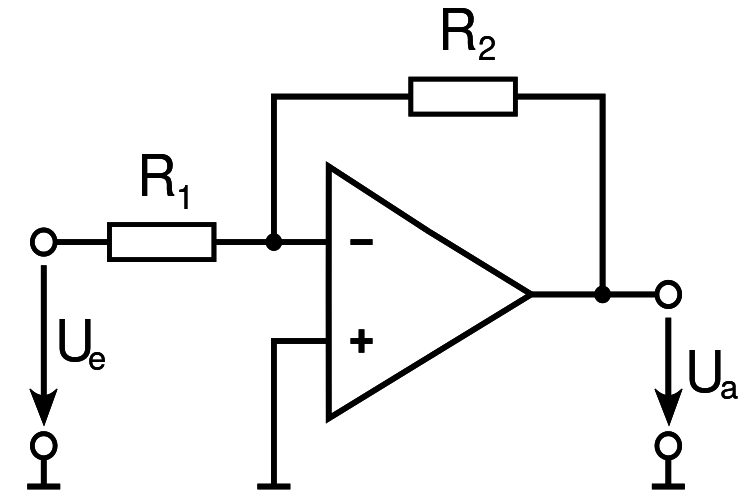
\includegraphics[width=\textwidth]{images/Inverting_Amplifier}
		\caption{Invertierender Verstärker}
	\end{subfigure}
	\begin{subfigure}{0.25\textwidth}
		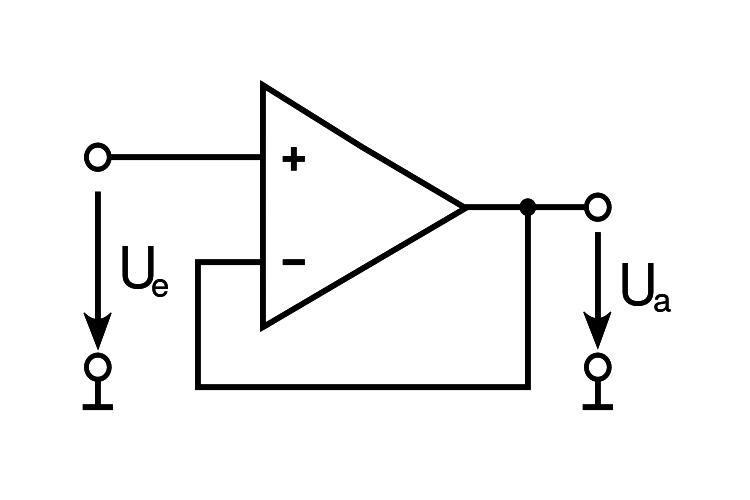
\includegraphics[width=\textwidth]{images/impedanzwandler}
		\caption{Impedanzwandler}
	\end{subfigure}
	\end{figure}
	
	\begin{figure}[h]
		\begin{subfigure}{0.25\textwidth}
		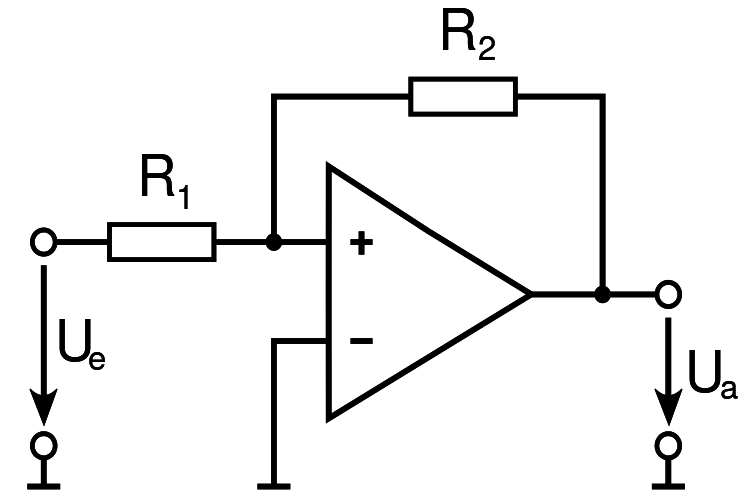
\includegraphics[width=\textwidth]{images/schmitt_noninv}
		\caption{Nicht invertierender Schmitt-Trigger}
		\end{subfigure}
		\begin{subfigure}{0.25\textwidth}
		\includegraphics[width=\textwidth]{images/schmitt_inv}
		\caption{Invertierender Schmitt-Trigger}
		\end{subfigure}
		\begin{subfigure}{0.25\textwidth}
		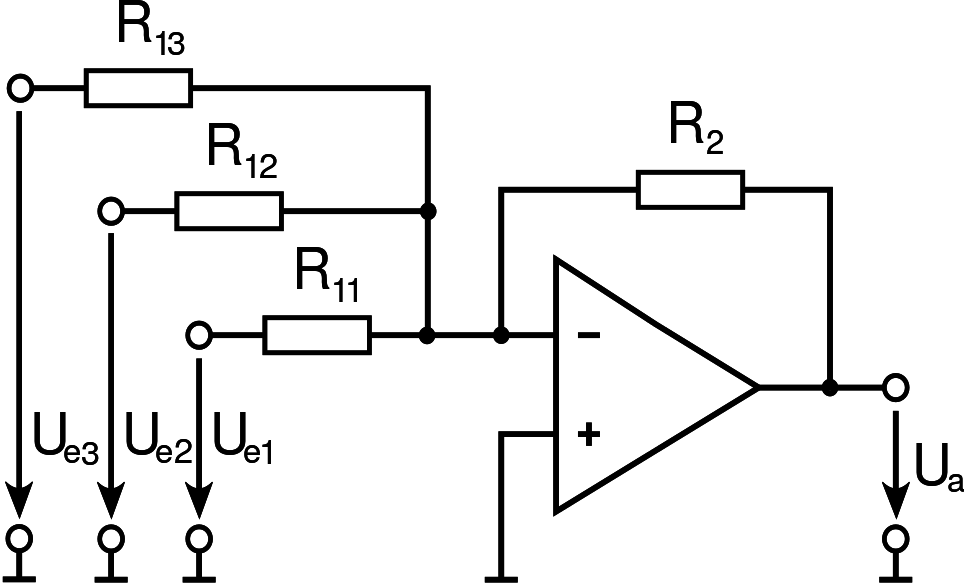
\includegraphics[width=\textwidth]{images/Inverting_Adder}
		\caption{Invertierender Addierer}
		\end{subfigure}
	\end{figure}
	\begin{figure}[h]
		\begin{subfigure}{0.25\textwidth}
		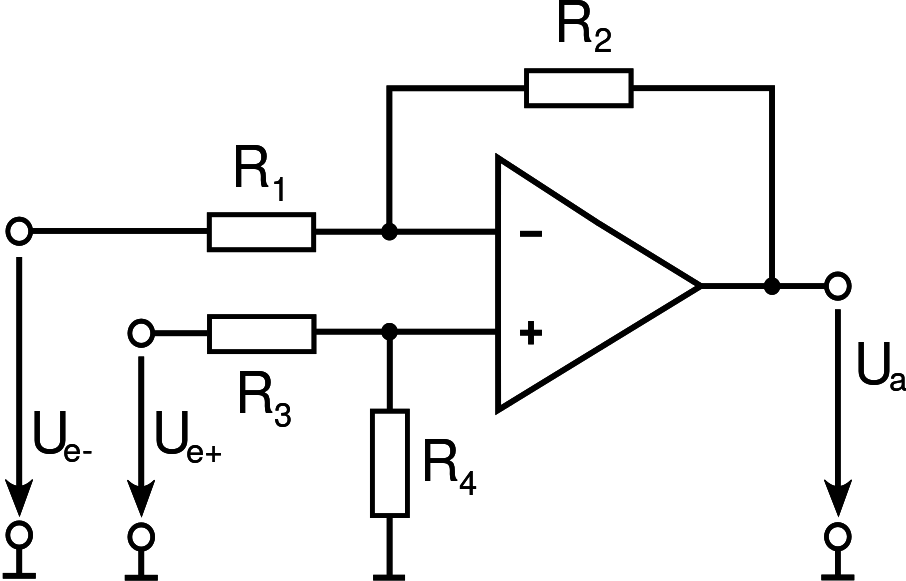
\includegraphics[width=\textwidth]{images/Differential_Amplifier}
		\caption{Subtrahierer (Differenzverstärker)}
		\end{subfigure}
		\begin{subfigure}{0.25\textwidth}
		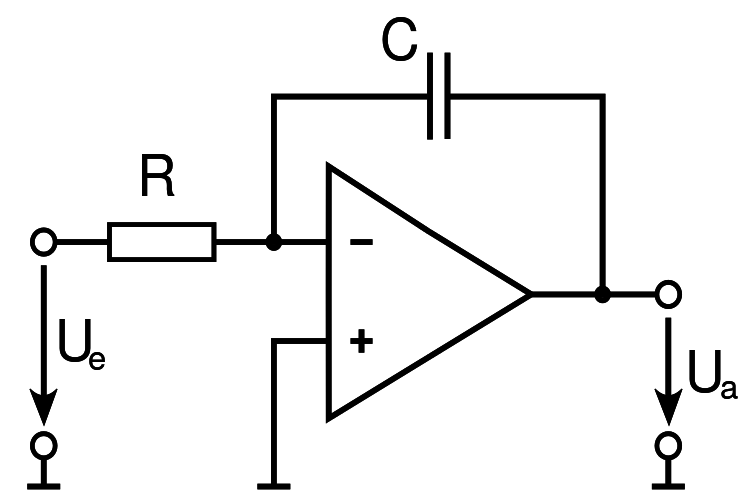
\includegraphics[width=\textwidth]{images/Integrating_Amplifier}
		\caption{Integrierer}
		\end{subfigure}
		\begin{subfigure}{0.25\textwidth}
		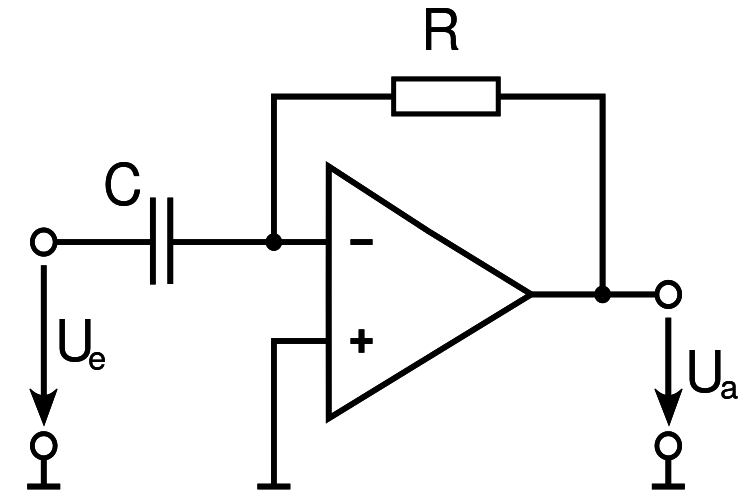
\includegraphics[width=\textwidth]{images/Differentiating_Amplifier}
		\caption{Differenzierer}
		\end{subfigure}
	\end{figure}
	\begin{figure}[h]
		\begin{subfigure}{0.25\textwidth}
		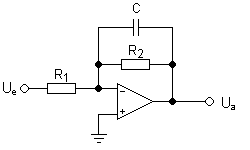
\includegraphics[width=\textwidth]{images/Aktiver_Tiefpass}
		\caption{Tiefpass}
		\end{subfigure}
		\begin{subfigure}{0.25\textwidth}
		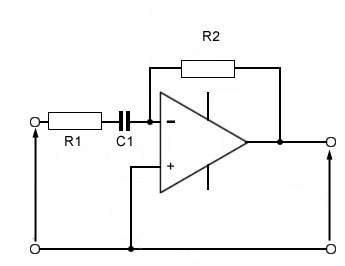
\includegraphics[width=\textwidth]{images/aktiver_hochpass}
		\caption{Hochpass}
		\end{subfigure}
		\begin{subfigure}{0.25\textwidth}
		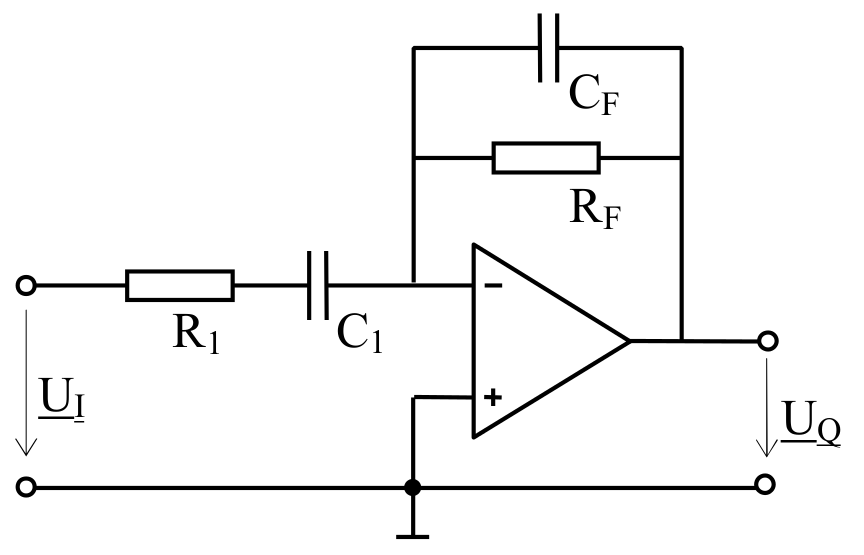
\includegraphics[width=\textwidth]{images/Bandpass}
		\caption{Bandpass}
		\end{subfigure}
	\end{figure}
\clearpage
	\begin{figure}[h]
		\begin{subfigure}{0.25\textwidth}
		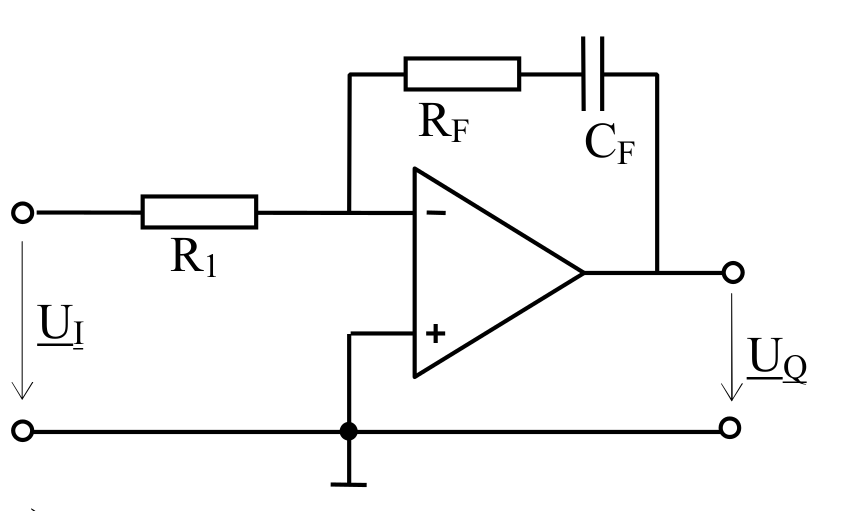
\includegraphics[width=\textwidth]{images/pi-regler}
		\caption{P-I-Regler}
		\end{subfigure}
	\end{figure}


	\subsection{Formeln}
		\begin{table}[h]
		\begin{tabularx}{\textwidth}{XXXX}
		& Nicht inv. Verst. & Inv. Verst. & Impedanzwandler\\
		\toprule
		Verstärkung & $V=\frac{u_{\mathrm{a}}}{u_{\mathrm{e}}}=1+\frac{R_2}{R_1}$ & $V=\frac{u_{\mathrm{a}}}{u_{\mathrm{e}}}=-\frac{R_2}{R_1}$ &1\\
		\midrule
		Eingangswiderstand & $\rightarrow \infty$ & $\approx R_1$ & $\rightarrow \infty$\\
		\bottomrule
		\end{tabularx}
		\end{table}
		
		\begin{table}[h]
		\begin{tabularx}{\textwidth}{XXX}
		Schaltung & Ausgangsspannung & Verstärkung / Zusätze\\
		\toprule
		Schmitt-Trigger (inv.) & $U_{\mathrm{S}1,2}=\frac{U_{\mathrm{QM}\pm}\cdot R_1+U_{\mathrm{Ref}}\cdot R_2}{R_1+R_2}$
		& $\Delta U_{\mathrm{Hyst}}=\frac{2U_{\mathrm{a}}R_1}{R_1+R_2}$\\
		\midrule
		Inv. Verst. & $U_{\mathrm{a}}=-U_{\mathrm{e}}\frac{R_2}{R_1}$ 
		& $V_{\mathrm{U}}=\frac{U_{\mathrm{a}}}{U_{\mathrm{e}}}=-\frac{R_2}{R_1}$\\
		\midrule
		Nicht inv. Verst. & $U_{\mathrm{a}}=U_{\mathrm{e}}\cdot\left(1+\frac{R_2}{R_1}\right)$ 
		& $V_{\mathrm{U}}=\frac{U_{\mathrm{a}}}{U_{\mathrm{e}}}=1+\frac{R_2}{R_1}$\\
		\midrule
		Addierer & $U_{\mathrm{a}}=-\left(\sum_{i=1}^3 U_{\mathrm{e}i}\cdot\frac{R_2}{R_{1i}}\right)$ 
		& $V_{\mathrm{U}}=-\frac{R_2}{R1} \Leftrightarrow R_i=R_1$\\
		\midrule
		Subtrahierer & $U_{\mathrm{a}}=$ & \\
		& $\left(U_{\mathrm{e}+}\cdot\frac{R_1+R_2}{R_3+R_4}\cdot\frac{R_4}{R_1}-U_{\mathrm{e}-}\cdot\frac{R_2}{R_1}\right)$ &\\
		\midrule
		Integrierer & $u_{\mathrm{a}}=-\frac{1}{RC}\int u_{\mathrm{e}} \mathrm{d}t$ 
		& $|V_{\mathrm{U}}|=\frac{\hat{u}_{\mathrm{a}}}{\hat{u}_{\mathrm{e}}}=\frac{1}{\omega RC}=f(\omega)$\\
		\midrule
		Differenzierer & $u_{\mathrm{a}}=-RC\cdot\frac{\mathrm{d}u_{\mathrm{e}}}{\mathrm{d}t}$ &
		$|V_{\mathrm{U}}|=\frac{\hat{u}_{\mathrm{a}}}{\hat{u}_{\mathrm{e}}}\approx\omega RC=f(\omega)$\\
		\midrule
		Tiefpass & $\underline{U}_{\mathrm{a}}=-\underline{U}_{\mathrm{e}}\frac{\underline{Z}_2}{\underline{Z}_1}$ 
		& $\left|\frac{V_{\mathrm{U}}(\omega)}{V_{\mathrm{U}}(0)}\right|=\frac{1}{\sqrt{1+\Omega^2}}$\\
		& $=-\underline{U}_{\mathrm{e}}\frac{R_2}{R_1}\frac{1}{1+j\omega R_2C}$ & $\Omega=\frac{\omega}{\omega_{\mathrm{G}}} \& \omega_{\mathrm{G}}=\frac{1}{R_2C}$\\
		\midrule
		Hochpass & $\underline{U}_{\mathrm{a}}=-\underline{U}_{\mathrm{e}}\frac{\underline{Z}_2}{\underline{Z}_1}$ 
		& $\underline{U}_{\mathrm{a}}=-\underline{U}_{\mathrm{e}}\frac{R_2}{R_1}\frac{1}{1-j\left(\frac{1}{\Omega}\right)}$ \\
		& $=-\underline{U}_{\mathrm{e}}\frac{R_2}{R_1}\frac{j\omega R_1C}{1+j\omega R_1C}$ & $\Omega=\frac{\omega}{\omega_{\mathrm{G}}}\&\omega_{\mathrm{G}}=\frac{1}{R_1C}$ \\
		\midrule
		PI-Regler & $\underline{U}_{\mathrm{a}}=\underline{U}_{\mathrm{e}}\left(-\frac{R_2}{R_1}+j\frac{1}{\omega C R_1}\right)$ &\\
		\bottomrule
		\end{tabularx}
		\end{table}

		\begin{table}[h]
		\begin{tabular}{lll}
		$U_{\mathrm{e}}\dots$ Eingangsspannung & $U_{\mathrm{a}}\dots$ Ausgangsspannung & $U_{\mathrm{S}}\dots$ Schaltschwelle\\
		$\Delta U_{\mathrm{Hyst}}\dots$ Hysterese & $\omega_{\mathrm{G}}\dots$ Grenzkreisfrequenz & $\Omega\dots$ Normierte Frequenz\\
		\end{tabular}
		\end{table}
\clearpage
